\documentclass[10pt, titlepage]{report}

\usepackage[utf8]{inputenc}
\usepackage[T1]{fontenc}
\usepackage[francais]{babel}

%Caractères spéciaux

\usepackage{lmodern}
\usepackage{amsmath}
\usepackage{amssymb}
\usepackage{mathrsfs}

\usepackage{eurosym} %insertion signe euro
\usepackage{graphicx} %insertion d'images
\usepackage{fancyhdr} %en-tete et pied de page

\title{\bsc{cahier des charges}\\Projet flight arena}
\author{mr cube :\\
Vincent \bsc{Rospini-Clerici},\\
Guillaume \bsc{Rebut}\\
%Nikolas \bsc{Miletic}\\
chef de projet : Arthur \bsc{Remaud}}
\date{16 janvier 2015}

\pagestyle{fancy}
\fancyhead{}
\fancyfoot{}
\lhead{Rapport de la première soutenance}
\rhead{Projet Flight Arena}
\lfoot{mr cube}

\begin{document}

\maketitle
\renewcommand{\contentsname}{Sommaire}
\renewcommand{\chaptername}{Partie}

\tableofcontents

\chapter{Modification du cahier des charges}
Suite au départ de Nikolas Miletic en S1\#, nous avons dû modifier le cahier des charges pour réajuster le budget et répartir à nouveau les tâches entre les trois membres restant.\\

Au niveau du budget, en terme de matériels, nous sommes passé de 3800 \euro à 2100 \euro. Le budget total est donc maintenant de 5397,29 \euro à 3697,29 \euro.\\

Pour la répartition du travail, le script a été confié à Arthur, Guillaume se charge entièrement du gameplay. Nous avons cependant pris du retard pour le son et la gestion des données. Le son a été pris sur internet alors que nous avions prévu de le faire nous-même. La gestion des données n'a quasiment pas été commencée : il n'y a pas de gestion de munitions ni d'affichage de la vie.\\

Pour les soutenances à venir, nous avons renoncé à faire le son, mais nous devrons nous rattraper pour les données afin d'avoir au moins des sauvegardes. Nikolas devait aussi s'occuper de l'I.A et du site web. C'est donc Guillaume et Arthur qui vont faire l'I.A et le site web sera construit par toute l'équipe.\\

\chapter{Retard/Avance par rapport au cahier des charges}
Le retard que nous avons par rapport aux prévisions du cahier des charges sont principalement causées par le départ d'un membre. Si nous regardons ce que nous nous avions fixé par personne, nous sommes dans les temps. 

\section{Retards}

\paragraph{Son :}
Nous avons pris la musique du menu sur internet au lieu de la faire par nos propres moyens : il s'agit de Captain America March. Pour le son des tirs, nous avons pris un bruitage du jeu Pinball sur Windows XP.

\paragraph{Gestion des données :}
Il n'y pas pour l'instant de gestion des données. Il n'y a pas de sauvegardes ou de munitions, et la vie ne s'affiche pas à l'écran. Le menu option ne comporte que la modification du volume du jeu.

\section{Avance}

\paragraph{Gameplay :}
Le gameplay est plus avancé que ce que nous espérions. Nous avons déjà un vaisseau opérationnel avec des contrôles qui fonctionnent assez bien.

\chapter{Travail par membre}
Nous allons vous décrire ce que chaque membre de l'équipe mr cube a fait pendant cette première période, avec leurs difficultés rencontrées et les techniques utilisées.

\section{Guillaume Rebut}

\section{Vincent Rospini-Clerici}

\section{Arthur Remaud}
Pendant cette première période, Arthur a fait tous les scripts en C\# du jeu et quelques modélisations 3D rapides avec blender.

\subsection{Scripts}
Tous les scripts en C\# du jeu ont été fait par Arthur grâce à des tutoriels sur internet. Il a entré les différentes saisies possibles du joueur, qui provoquent sur le vaisseau des translations avec la fonction $transform.Translate$ lorsque le joueur veut avancer ou des rotations avec la fonction $transform.Rotate$ lorsque le joueur veut tourner. Chacun peut donc aisément piloter le vaisseau pour éviter les obstacles. Il a aussi mis une touche pour tirer. \textit{Unity} crée une instance de la balle qui part droit devant. Elle disparait automatiquement au bout de quelques secondes, le temps d'au moins traverser le terrain, pour éviter d'avoir trop d'objets à la fois, ce qui provoquerait un ralentissement du jeu. \\

La principale difficulté rencontrée fut la gestion de l'inertie lorsque l'objet est touché par le décor. En effet, il peut rapidement partir en vrille et n'est plus maniable. Après des recherches sur internet, il est apparu que le problème venait du rigidbody et c'est la vélocité de celui-ci qu'il faut remettre à zéro à chaque fois.\\ \\

 Il a aussi fait les menus, en utilisant les propriétés GUI (Graphical User Interface) de \textit{unity}. Il a pris une police futuriste nommée \textit{airstrike}, et c'est lui qui a choisit la musique \textit{Captain America March} pour le menu qu'il connaissait auparavant puisqu'il l'a joué à la trompette. Mais pour plus de confort, on a mis la version officielle de la musique. Nous aimerions par la suite conserver ce genre de musique pour le jeu, avec des grands orchestres et des cuivres sonnant, comme on peut en avoir dans \textit{Star Wars}.\\

Il n'a pas réussi à intégrer les animations d'explosions faites dans \textit{unity}, car l'exportation depuis \textit{blender} échoue.

\subsection{Modélisation 3D}
Arthur a fait quelques objets rapidement sur blender pour le projet. Il a ainsi créé six vaisseaux et quatre bâtiments rapidement. Ils sont cependant assez laid et ne seront donc utilisé que pour le décor ou en personnage non joué, le vaisseau principal ayant été fait par Vincent.

Il a utilisé les même techniques que Vincent pour la modélisation, à savoir l'outil \textit{mirror} pour avoir des vaisseaux symétriques, et  l'UV-mapping pour faire les textures.

Il a fait ses textures lui-même avec photoshop plutôt que de les prendre en ligne. Elles sont donc par conséquent moins détaillées mais plus personnelles.\\ \\ \\

\begin{center}
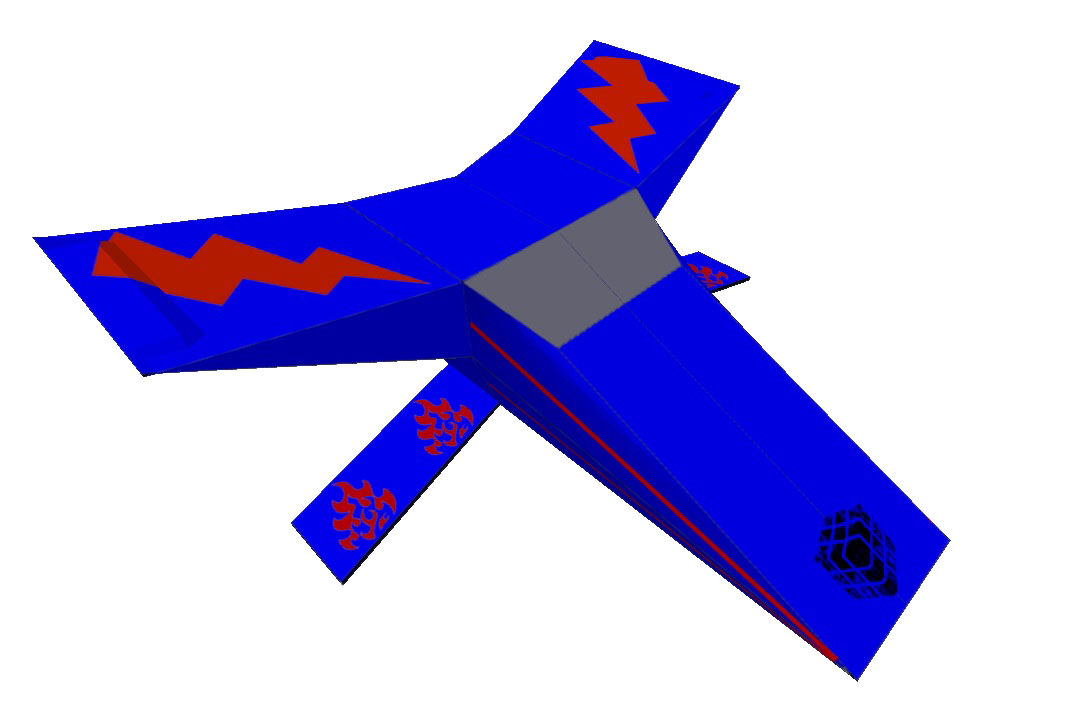
\includegraphics[height=6cm, width=9cm]{vaisseau arthur.jpg}\\
\end{center}


\chapter{Pour la prochaine soutenance}

Tout d'abord, nous allons améliorer le contenu : ajouts de vaisseaux, de niveaux, de bâtiments \dots
Le menu sera aussi complété, notamment dans les options et dans le choix de son vaisseau.\\

Mais surtout, la prochaine soutenance verra l'apparition des \textbf{I.A} et du \textbf{multijoueur en réseau local}. Cela augmentera considérablement le gameplay et l'intérêt du jeu.

\end{document}